\documentclass[12pt,fleqn]{article}\usepackage{../../common}
\begin{document}
Kesit Seviyeleri (Level Sets) ile İmaj Gruplamak 

Bir dijital resimdeki bir kümeyi, grubu ortaya çıkartmak (segmentation) için bir
teknik daha, kesit seviyeleri kullanmak. Grup bulmak derken resimdeki
diğerlerinden daha ayrı duran, bizim çıplak gözle gördüğümüz bir grubu
diğerlerinden ayırıp etrafındaki sınırlar çizmek, ve bunları otomatik
olarak yazılımın yapmasını sağlamak. 

Kesit seviyeleri tekniği her ne kadar dışarıdan bir eğriyi belli bir enerji
fonksiyonunu minimize ederek kümenin etrafında ``sarmalayan'' yılan (snake)
tekniğine benzese de, aslında daha derin ve kuvvetli özellikleri olan bir
yaklaşımdır. Yılan tekniğinde eldeki bir eğriyi bizzat değiştirerek grup
etrafını sarmalasına uğraşıyoruz. Kesit seviyeleri ile grubu tanımlayan manipüle
ettiğimiz sınıların kendisi değil bir yansımadan dolaylı elde edilen ama kendisi
daha yüksek boyutta olan başka bir fonksiyon.

Alttaki görüntüler daha iyi açıklayabilir,

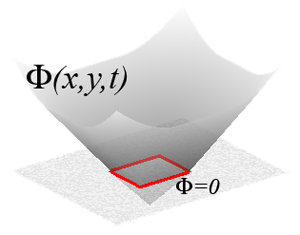
\includegraphics[width=20em]{compscieng_app50lset_02.png}

İmajın düzlemde olduğunu düşünürsek o görülen kırmızı çizgiler kesit seviyesi
($\phi=0$ için). İmaj düzlemi, ve kesit seviyesi iki boyutlu, manipüle edilen
ise üç boyutlu bir $\phi$ fonksiyonu, ve gruplamayı yapan bu fonksiyonun sıfır
kesit seviyesindeki kontur çizgileridir, yani $\phi(x,y,t) = 0$ ne ise gruplama,
küme (segment) odur.

Altta, değişen $\phi$'nin imaj düzlemindeki değişen kesit seviyesini görebiliyoruz.

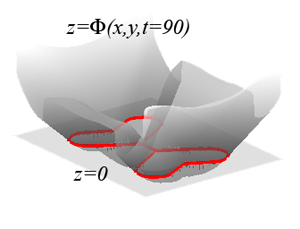
\includegraphics[width=20em]{compscieng_app50lset_01.png}

Peki $\phi$ fonksiyonunu imaj üzerindeki yakın duran pikselleri göz önüne alarak
(ki kesit seviyesi onların etrafını sarsın) nasıl değiştireceğiz? İşte kesit
seviyeleri matematiği burada devreye giriyor.

Ana yüzey fonksiyonu $\phi(x,y)$, ya da vektörel olarak $\phi(\vec{x})$, daha
basit $\phi(x)$ diyelim, bu yüzeyi $t$ ile parametrize edersek kesit seviyesini

$$
\phi(x(t), t) = 0
$$

ile tanımlarız. Üstteki eşitliği $t$ için elde edilen $x$ için $t$ anındaki
yüzeyin fonksiyonu olarak düşünebiliriz. Şimdi sıfır seviyesindeki kontur
eğrisinin değişimini takip etmek istediğimiz için [5], üstteki eşitliğin $t$'ye
göre değişiminin açılımını görmek istiyoruz. Hatırlarsak pozisyonun türevi
hızdır, ve eğer hızı bilirsek yüzeyin hareketini modelleyebiliriz.

$$
\frac{\partial \phi(x(t),t)}{\partial t} = 0
$$

Zincirleme Kuralını uygulayınca

$$
\frac{\partial \phi}{\partial x(t)} \frac{\partial x(t)}{\partial t} +
\frac{\partial \phi}{\partial t} = 0
$$

Tanım itibariyle $\partial \phi / \partial x(t)$ kısmi türev yüzeyimizin
gradyanı, bunu temel çok boyutlu Calculus'tan biliyoruz. Diğer notasyonu da
biraz kısaltınca

$$
\nabla \phi x_t + \phi_t = 0
$$

Üstte eğrinin hareketinin $\phi$'ye normal / dik olduğunu söylemiş olduk,
eğer yönü birim vektör olarak göstermek gerekirse, $\frac{\nabla \phi}{||\nabla \phi ||}$.
Şimdi hızın kendisi lazım, düzlemdeki yere bağlı olarak değişebilecek
bir $F$ kuvveti ile yönü çarparak yönsel hızı elde edebiliriz,
$x_t = F \frac{\nabla \phi}{||\nabla \phi ||} $. Yerine koyarsak,

$$
\nabla \phi F \frac{\nabla \phi}{||\nabla \phi ||}  + \phi_t = 0
$$

$$
F \frac{||\nabla \phi||^2}{||\nabla \phi ||}  + \phi_t = 0
$$

$$
F ||\nabla \phi||  + \phi_t = 0
$$

Biraz daha organize edince kesit seviyeleri denklemini elde ediyoruz.

$$
\phi_t = - F ||\nabla \phi|| 
$$

Bu bize yüzeyin değişim hızı $\phi_t$'yi veriyor.

Hesaplama

$\phi$'nin başlangıç değerlerini biliyorsak ve değişim hız formülünü baz alarak
hareket denklemini çözebiliriz / zamanda ileri doğru taşıyabiliriz. Yani bulmak
istediğimiz herhangi bir $t$ anındaki $\phi$. Hesabı yapmanın en basit yolu
Sonlu Farklar (Finite Differences) yöntemi ile.  Temel Calculus'tan hatırlarsak,

$$
f'(x) = \frac{f(x+\Delta x) - f(x)}{\Delta x}
$$

Bunu $\phi$ için uygularsak,

$$
\frac{\partial \phi(x(t),t)}{\partial t} =
\frac{\phi(x(t),t+\Delta t) - \phi(x(t),t)}{\Delta t}
$$

$$
\Delta t \phi_t = \phi(x(t),t+\Delta t) - \phi(x(t),t)
$$

$$
\phi(x(t),t+\Delta t) = \phi(x(t),t) + \Delta t \phi_t
$$

Şimdi $\phi_t$ için daha önce bulduğumuz formülü koyarsak,

$$
\phi(x(t),t+\Delta t) = \phi(x(t),t) - \Delta t F ||\nabla \phi|| 
$$

Böylece değişim fonksiyonunu elde etmiş olduk. Yapay Öğrenim konusunu
bilenlere üstteki formül tanıdık gelebilir, $\phi$ üzerinde $t$ bazlı
olarak gradyan inişi (gradient descent) yapmış oluyoruz bir bakıma.

$$
\phi' = \phi + \Delta t F ||\nabla \phi ||
$$

Not: Üstte $+\Delta t F$ var fakat türetimden $+\Delta t F$ gelmesi gerekiyor.
Eğer ilerideki kodda işareti değiştirsek bunun işlemeyeceğini görürdük, artı
olması gerekiyor. Bu gradyan tanımıyla alakalı, fakat istenen işarete direk
erişmek için sonlu farklar başlangıcında ufak bir değişiklikle yine artı
elde edebiliriz.

Şimdi $F$ konusuna gelelim; bu $F$'nin seçilmesi kesit seviyesi yöntemimize
direk etki edecektir. Sonuç olarak eğriyi belli bir yönde, ve hızda ittiren
``kuvvet'' budur. $F$ resmin her noktasında tanımlı bir nevi hız, kuvvet
alanı (velocity field) olarak görülebilir, her noktada bize $\phi$'nin
hareketinin yönünü ve büyüklüğünü verir.

O zaman düşünürsek, imajda gruplama yapmak istiyoruz, ve alttaki gibi bir resim
var diyelim,

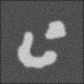
\includegraphics[width=10em]{twoObj.png}

$F$'nin ortadaki objenin sınırlarına kadar yüksek olmasını ama sınırlarda çok az
hatta sıfır olmasını isteyebiliriz, değil mi? Bu dolaylı olarak obje tanımlamayı
gerçekleştirecektir, çünkü $\phi$ yüzeyi objeye gelinceye kadar hızla
ilerleyecek, ardından obje çevresine geldiği noktalarda yavaşlayacaktır, ve yan
etki olarak kesit seviyesi nesneyi sarmalamış olur, ve bu noktada gruplamayı
bitmiş kabul edebiliriz.

$F$'yi o zaman direk imajın kendisinden hesaplayalım, ve onu bir nevi kenar
algılayıcı (edge detector) olarak görelim. Eh en basit kenar bulucu gradyan
olduğuna göre imajın gradyanını almak yeterli olacaktır. $I$ imajı için $g$
gradyanı [6],

$$
g(I) = \frac{1}{1  + || \nabla I ||^2}
$$

Hepsini bir araya koyunca alttaki kod yazılabilir,

\begin{minted}[fontsize=\footnotesize]{python}
from skimage import color, io
import scipy.ndimage

def grad(x):
    return np.array(np.gradient(x))

def norm(x, axis=0):
    return np.sqrt(np.sum(np.square(x), axis=axis))

def stopping_fun(x):
    return 1. / (1. + norm(grad(x))**2)

def default_phi(x):
    # phi yuzeyini imaj disindaki 5 piksel genisligindeki bantta 1
    # bant icinde ise -1 olarak tanimliyoruz
    phi = np.ones(x.shape[:2])
    phi[5:-5, 5:-5] = -1.
    return phi

img = io.imread('twoObj.bmp')
img = color.rgb2gray(img) # grilestir
img = img - np.mean(img) # ortalamayi cikart
# puruzsuzlestirme uygula yanyana pikseller daha benzer olsun
img_smooth = scipy.ndimage.filters.gaussian_filter(img, sigma=2)

F = stopping_fun(img_smooth)

dt = 1.
n_iter = 100
phi = default_phi(img)
for i in range(n_iter):
    dphi = grad(phi)
    dphi_norm = norm(dphi)
    dphi_t = F * dphi_norm
    phi = phi + dt * dphi_t
    if i%10==0:
        plt.imshow(img,cmap = 'gray')
        plt.contour(phi, levels=[0],colors=['red'])
        plt.savefig('img2/out-%03d.png' % i)
        plt.close()
\end{minted}

İşlemden seçilmiş üç kare alttadır,

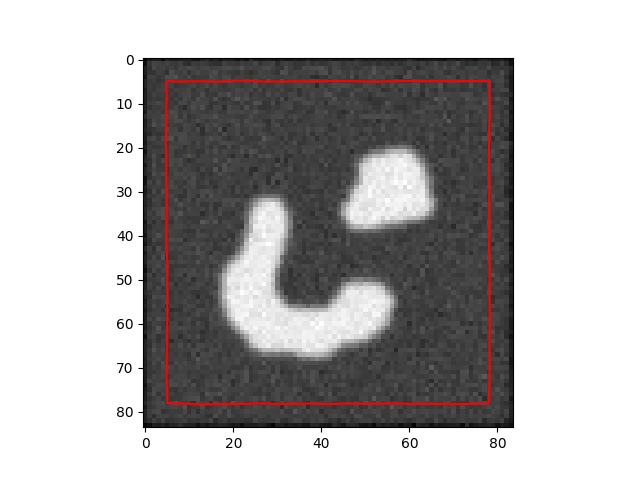
\includegraphics[width=12em]{img2/out-000.png}
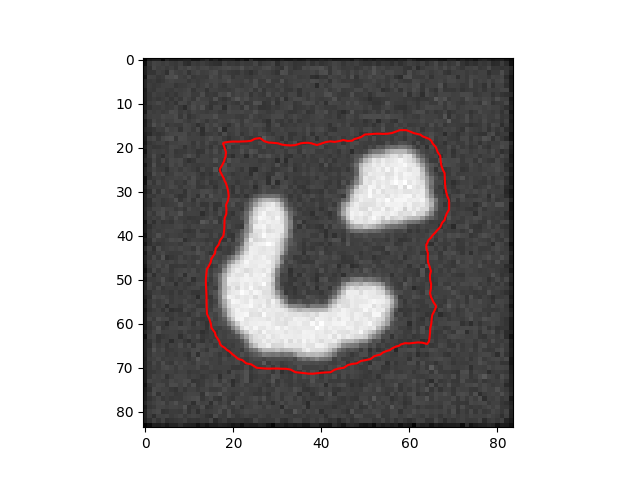
\includegraphics[width=12em]{img2/out-020.png}
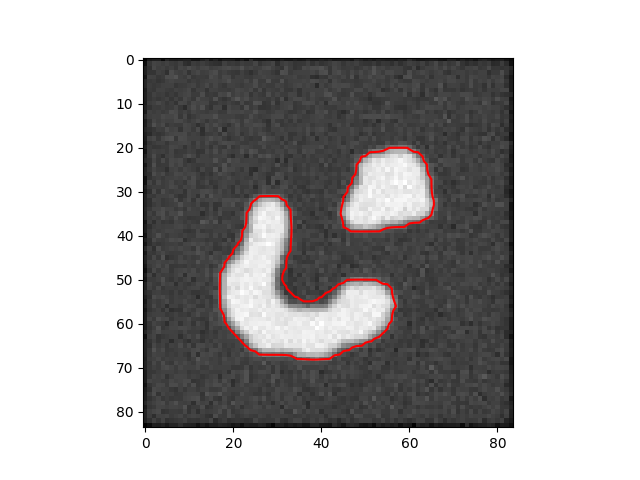
\includegraphics[width=12em]{img2/out-090.png}

Kesit seviyeleri tekniğinin faydalarının görmek zor değil; üç boyutlu fonksiyonu
daha esnek yönlerde değiştirebileceğimiz için onu düzlemdeki yansımaları
birbirinden kopuk duran (ama alakalı) obje gruplarını bile bulup çıkartabilir.


\newpage

Eski Yazı

Eğim (Curvature)

Kesit seviyeleri tekniğinde bir eğri normal formda değil, dolaylı
(implicit) bir fonksiyon ile $F(x,y) = 0$ olarak gösterilir. Bu fonksiyonun
tam diferansiyelini alırsak,

$$ dF = F_x dx + F_y dy = 0  $$

$$ dy = -F_x / F_y dx  $$

$$ y' = \frac{dy}{dx} = -F_x / F_y = f'(x) = \frac{df}{dx} $$

Burada bir faraziye daha var, o da aslında ilk verilen formülde olmasa bile
$y=f(x)$ olarak kabul etmemiz, yani $F(x,y)$ nasıl bir formül olursa olsun,
$y$'nin $x$'leri içerecek şekilde tekrar düzenlenebileceğini farz etmemiz,
böylece $F(x,f(x))$ olabileceğini söylemiş oluyoruz [4].

Şimdi $y'$ ifadesinin türevini bir daha alalım. Yukarıdaki $y'$ formülünde
en sağ taraf bir bölme işlemi içerdiği için burada Calculus'un Bölümler
Kuralını (Quotient Rule) uygulamamız lazım (detaylar için Bölüm Kuralı
yazısına bakınız). Bu kural şöyle gösterilir:

$$ \frac{d}{dx}\bigg(\frac{u}{v}\bigg) = 
\frac{\displaystyle \frac{v du}{dx} - \frac{u dv}{dx}}{v^2} $$

Bölümler Kuralı için $u$ ve $v$ tanımları nedir? 

$$ u = -F_x(x,f(x))  $$

$$ v = F_y(x,f(x)) $$

O zaman

$$ 
v \frac{du}{dx} = F_y \frac{dF_x}{dx} 
\mlabel{1}
$$

$$
u \frac{dv}{dx} = -F_x \frac{dF_y }{dx} 
\mlabel{2}
$$

Bunlardan mesela $dF_x/dx$ üzerinde Zincirleme Kanunu (Chain Rule) uygulamak
lazım (bu kural tam integral kuralının bir sonucu). 

$$ \frac{d F_x(x,f(x)) }{dx} = \frac{\partial F_x}{\partial  x}(x,f(x))+\frac{\partial F_x}{\partial y}\frac{df}{dx}\\ $$

$$
= F_{xx}(x,f(x))+F_{xy}(x,f(x))f'(x) 
\mlabel{3}
$$

$$
\frac{d F_y(x,f(x)) }{dx} =  F_{xy}(x,f(x))+F_{yy}(x,f(x))f'(x) 
\mlabel{4}
$$

Zincirleme Kanunu niye üstteki şekilde açıldı? Tam Diferansiyeli bir daha
hatırlayalım:

$$ df = \frac{\partial f}{\partial x} dx + \frac{\partial f}{\partial y} dy  $$

$$ \frac{df}{dx} = \frac{\partial f}{\partial x} \frac{dx}{dx} + \frac{\partial f}{\partial y} \frac{dy}{dx}  $$

$$ \frac{df}{dx} = \frac{\partial f}{\partial x} + \frac{\partial f}{\partial y} \frac{dy}{dx}  $$

O zaman formüller (1) (2) (3) ve (4) bir araya konulursa,

$$ y '' = - \frac{F_yF_{xx} - F_y F_{xy}\frac{F_x}{F_y} - F_xF_{xy} + F_xF_{yy}\frac{F_x}{F_y}}{F_y^2}\\ $$

$$ y '' = - \frac{F_yF_{xx} - F_{xy}F_x - F_xF_{xy} + \frac{F_x^2F_{yy}}{F_y}}{F_y^2} $$

Üstteki bölümün hem bölen, hem bölünen terimlerini $F_y$ ile çarparsak, ve
sadeleştirirsek

$$ y '' = - \frac{F_y^2F_{xx} - 2F_{xy}F_xF_y + F_x^2F_{yy}}{F_y^3} $$

Şimdi surada [2] türetimi gösterilen eğim  formülüne
bakalım. Not: Eğer

$$ \kappa = \frac{x'y''-y'x''}{\bigg(x'^2 + y'^2 \bigg)^{3/2}} $$

formülünün alttaki formüle nasıl dönüştüğü tam anlaşılır değilse,
hatırlayalım ki, $y=f(x)$, ve $x'=1$, ve $x'' = 0$.

Bu formülün Courant [1] sf. 231'de benzer bir formunu görüyoruz (Bu arada o
karmaşık formül yerine yaklaşıksal olarak hesaplama sırasında sadece $f''$
kullanmak ta mümkün [3, giriş bölümü])

$$ \kappa = \frac{f''}{(1+f'^2)^{3/2}} $$

Bu formüldeki $f''$ yani $y''$ için üstte bulduğumuz sonucu, $f'$ yani $y'$
için bu yazının başındaki formülü koyarsak,

$$ 
\kappa = \frac
{-\frac
{\displaystyle F_y^2F_{xx} - 2F_{xy}F_xF_y +  F_x^2F_{yy}}{\displaystyle F_y^3}}
{(1+f'^2)^{3/2}} 
$$  

Bölen kısmı nedir?

$$ (1+f'^2)^{3/2} = \bigg( 1 + \bigg(\frac{-F_x}{F_y}\bigg)^2 \bigg)^{3/2}  $$

$$ = \bigg( 1 + \frac{F_x^2}{F_y^2} \bigg)^{3/2}  $$

$$ = \bigg( \frac{F_y^2 + F_x^2}{F_y^2} \bigg)^{3/2}  $$

$$ = (F_y^2 + F_x^2)^{3/2}(F_y^{-2})^{3/2}  $$

$$ = (F_y^2 + F_x^2)^{3/2}F_y^{-6/2}  $$

$$ = (F_y^2 + F_x^2)^{3/2}F_y^{-3} $$

Yerine koyarsak,

$$ 
\kappa = \frac{\displaystyle
- \frac{F_y^2F_{xx} - 2F_{xy}F_xF_y + F_x^2F_{yy}}{F_y^3}}
{(F_y^2 + F_x^2)^{3/2}F_y^{-3}}
 $$

$F_y^{-3}$ ve $F_y^{3}$ birbirlerini iptal ederler ve sonuç:

$$
\kappa = \frac{F_y^2F_{xx} - 2F_{xy}F_xF_y +
    F_x^2F_{yy}}{(F_y^2 + F_x^2)^{3/2}}
\mlabel{5}
$$

Üstteki ünlü eğim  formülüdür. 

Bu eğim formülünün diğer bir şekli şöyledir ($F$ yerine $\phi$ kullanırsak)

$$ \kappa = \bigtriangledown \cdot \frac{\bigtriangledown \phi}{|\bigtriangledown \phi|} $$

Bunun okunuş şekli ``birim normal gradyanın uzaklaşım ölçüsü (divergence of the
unit normal gradient)'' şeklindedir. Acaba bu formül, (5). formül ile
uyumlu mu?

$$ \kappa = \nabla \cdot \frac{\nabla \phi}{|\nabla \phi|}  $$

$$ = \nabla \cdot \frac{(\phi_x,\phi_y)}{\sqrt{\phi_x^2+\phi_y^2}} $$

$$ = \left(\partial_x \frac{\phi_x}{\sqrt{\phi_x^2+\phi_y^2}}\right)+ 
\left(\partial_y \frac{\phi_y}{\sqrt{\phi_x^2+\phi_y^2}}\right)  $$

$$ = \frac{\phi_{xx}}{\sqrt{\phi_x^2+\phi_y^2}} - \frac{\phi_x (\phi_x\phi_{xx}+\phi_y\phi_{xy})}
{(\phi_x^2+\phi_y^2)^{3/2}} +
\frac{\phi_{yy}}{\sqrt{\phi_x^2+\phi_y^2}} - \frac{\phi_y(\phi_x\phi_{xy}+\phi_y\phi_{yy})}
{(\phi_x^2+\phi_y^2)^{3/2}}  $$

$$ = \frac{\phi_{xx}(\phi_x^2+\phi_y^2) - \phi_x
  (\phi_x\phi_{xx}+\phi_y\phi_{xy}) +\phi_{yy}(\phi_x^2+\phi_y^2) -
  \phi_y(\phi_x\phi_{xy}+\phi_y\phi_{yy})}{(\phi_x^2+\phi_y^2)^{3/2}} $$

$$ = \frac{\phi_{xx}\phi_y^2 - 2\phi_x\phi_y\phi_{xy} + \phi_{yy}\phi_x^2}{(\phi_x^2+\phi_y^2)^{3/2}}  $$

Bu formül bizim (5). formül ile tıpatıp aynı.

Üstteki işlemlerde uzaklaşım ölçüsü (divergence) operatörü $\nabla \cdot$
ile gradyan operatörü $\nabla$ arasındaki farkı belirtelim: $\nabla \cdot$
operatörü $F(x,y)$ üzerinde kısmi türevlerin toplamını verir, yani bir
skalar tek sayı döndürür. Gradyan ise her bir elemanı bir kısmi türeve
tekabül eden bir {\em vektör} geri getirir.

Python Numpy kodlaması bağlamında, daha önce {\em Kesit Seviyeleri} yazısında
ayrıksal olarak bir \verb!phi! değişkeni içindeki bir fonksiyon üzerinde
eğimselliği şöyle hesaplamıştık:


\begin{minted}[fontsize=\footnotesize,linenos,xleftmargin=1cm]{python}
gradPhiY, gradPhiX = np.gradient(phi)
absGradPhi=np.sqrt(gradPhiX**2+gradPhiY**2)                               

normGradPhiX=gradPhiX/(absGradPhi+(absGradPhi==0))
normGradPhiY=gradPhiY/(absGradPhi+(absGradPhi==0))

divYnormGradPhiX, divXnormGradPhiX=np.gradient(normGradPhiX)
divYnormGradPhiY, divXnormGradPhiY=np.gradient(normGradPhiY)
                       
K = divXnormGradPhiX + divYnormGradPhiY
\end{minted}

Bu satırların $\nabla \cdot \frac{\nabla \phi}{|\nabla \phi|}$ ifadesiyle
birebir uyum gösterdiğini herhalde görebiliyoruz. Satır 1, $\nabla \phi$
ifadesidir. Satırlar 4-5 $\frac{\nabla \phi}{|\nabla \phi|}$ işlemini
gerçekleştiriyor, gradyanı onun uzunluğuna (magnitude) bölerek onu birim vektörü
haline getiriyor. Satırlar 7-10 tekrar sonucun gradyanını bir daha alıyor, ama
bu sefer hesapsal kısmi türevleri birbiriyle topluyor, böylece uzaklaşım ölçüsü
(divergence) hesaplanmış oluyor. Tüm bu işlemlerin sonucu eğimsellik $\kappa$
oluyor.

Dikkat edilirse Python kodundaki K yani $\kappa$, N x N boyutlu bir matristir,
bu mantıklı çünkü $\kappa$ hesabı için kullandığımız $F_x$, $F_y$ gibi
türevler aslında $F_x(x,y)$, $F_y(x,y)$ formüllerine sahipler, yani her $x,y$
kombinasyonu için farklı bir sonuç döndürebilirler. Bu sebeple K yani $\kappa$
$\phi$ fonksiyonunun her $x,y$ noktası için tanımlıdır. 

Bazen literatürde $\nabla \cdot$ yerine $div(..)$ kullanıldığını görebilirsiniz,
bu operatörlerin ikisi de aynıdır.

Kesit Seviyeleri, Kenar Bazlı İmaj Gruplamak

Bir dijital imajı renklere, objelere göre belli parçalara bölmek
(segmentation) için, matematiksel bir formül kullanmak iyi çözümlerden
biridir. Bunu yapmanın bazı yolları var. Basitleştirerek bir örnek
verelim: diyelim ki gruplama için elimizdeki formül bir yuvarlak
formülü $x^2+y^2 - c = 0$, ki $c$ bir sabit. Bu formülü x ve y
kordinatları üzerinde bastığımız zaman radius'u $\sqrt{c}$ olan bir
çember elde ederiz. Gruplama için bu çemberi büyütüp
küçültebildiğimizi farzedelim, çember imaj üzerindeki istediğimiz
bölüme en iyi uyduğu anda gruplamayı başarılı olarak kabul ediyoruz.

Fakat problem şurada: eğer imajda birden fazla grup var ise, o zaman
birden fazla çember gerekecektir, bu sefer algoritmik olarak üstteki
formülü ikinci, üçüncü kere yaratmamız, ve o formüllerin o gruplara
uyumunu ayrı ayrı takip etmemiz gerekirdi. Ya da diyelim ki özyineli
(iterative) bir uydurma işlemi takip ediyoruz, bu işlem sırasında
belki iki çemberin birleşmesi gerekse, o zaman iki formülü silip,
yerine yenisini oluşturmakla uğraşmak gerekli olacaktı. Bunlar hem
matematiksel, hem kodlama açısından külfet oluşturacaktır.

Kesit Seviyeleri kavramını kullanarak bu işi daha
basitleştirebiliriz. Diyelim ki bölme görevini yapan $\phi$ adli
fonksiyonumuzu 2 boyutlu olmak yerine 3 boyutlu eksende tanımladık,
ve, 2 boyutta bölme yapma görevini onun bir kesitine verdik. Kesit
derken, alttaki üç boyutlu fonksiyonu yatay olarak bir noktadan
``kestiğimizi'' farz ediyoruz, ve o kesit üzerinde düşen $\phi$
değerlerine bakıyoruz.

Bakıç açışımızı, tanımlamamızı değiştirerek, bazı avantajlar elde
etmeyi umuyoruz aslında. Altta iki tane $\phi$ fonksiyonu ve onların
altında kesitlerini görebiliriz.


Kesit Seviyeleri tekniğini kullanarak elde ettiğimiz avantaj nedir?
Artık sadece \textbf{tek} bir $\phi$ fonksiyonu kullanarak 2 boyutlu
imajımız üzerinde birbirinden ayrı gruplamalar yaratabiliyoruz. Bu
gruplar birbiri ile birleşebilir, ayrılabilir, bu artık bizi
ilgilendirmiyor. Biz sadece 3. boyuttaki $\phi$ fonksiyonunu
değiştirmekle uğraşacağız, imaj üzerindeki gruplamalar ise o
fonksiyonun 2. boyuta yansıması (projection) üzerinden kendiliğinden
gerçekleşecekler.

Matematiksel olarak $\phi$ fonksiyonunu nasıl temsil ederiz? $\phi$
fonksiyonu $x$, $y$, boyutlarını alıp bize bir üçüncü $z$ boyutu
döndürmeli, ayrıca bu fonksiyonu imajı parçalarına ayırma işlemini
gerçekleştirmek için kademeli olarak değiştirmeyi planladığımıza göre,
o zaman bir $t$ değişkeni de gerekiyor. Yani $\phi(x,y,t)$
fonksiyonu. Gruplama için kullanılacak kesiti ise sıfır kesiti olarak
alalım, yani $\phi(x,y,t) = 0$. Doğal olarak

$$ \frac{d}{dt}(\phi(x,y,t) = 0) = 0 $$

Şimdi $x$, ve $y$ değişkenlerinin zaman göre değişimini formüle bir
şekilde dahil etmek lazım. Bunun için sıfır kesit seviyesi üzerinde
bir parçacık hayal edilir, ve bu parçacığın gittiği yol $x(t)$, ve
$y(t)$ olarak tanımlanır. O zaman

$$ \frac{d}{dt}(\phi(x(t),y(t),t)) = 0 $$

Tam diferansiyel formülünden hareketle:

$$ 
d(\phi(x(t),y(t),t) = 
\frac{\partial \phi}{\partial x}dx + 
\frac{\partial \phi}{\partial y}dy + 
\frac{\partial \phi}{\partial t}dt  = 0
 $$

$$ 
\frac{d(\phi(x(t),y(t),t))}{dt} = 
\frac{\partial \phi}{\partial x}\frac{dx}{dt} + 
\frac{\partial \phi}{\partial y}\frac{dy}{dt} + 
\frac{\partial \phi}{\partial t} = 0
 $$

$$
 = 
\frac{\partial \phi}{\partial x}\frac{dx}{dt} + 
\frac{\partial \phi}{\partial y}\frac{dy}{dt} + 
\phi_t = 0
\mlabel{1}
$$

Temsilen daha kısa bir işaret kullanmak gerekirse, $\bigtriangledown$
ile $\phi$'nin gradyanını (gradient) alarak, elde edilecek vektörün
nokta çarpımını kullanabiliriz.  O zaman formül (1) daha kısa
olarak:

$$ \phi_t + \bigtriangledown \phi \cdot \vec{V} = 0 $$

olarak temsil edilebilir, ki

$$ \bigtriangledown \phi = \bigg(
\frac{\partial \phi}{\partial x},
\frac{\partial \phi}{\partial y} \bigg)
 $$

$$ \vec{V} = \bigg(
\frac{dx}{dt} ,
\frac{dy}{dt} \bigg)
 $$

İki vektörün nokta çarpımı bilindiği gibi sırayla her iki vektörün
sırasıyla uyan elemanlarının birbirleri ile çarpılması ve o
çarpımların toplanmasıdır.

$\vec{V}$ vektörü neyi temsil eder? Formüle göre bu vektör $\phi$'nin
üzerindeki değişimi etkiliyor, ve bu değişimler $t$'nin değişimine
göre tanımlandığına göre bu değerler ``hız'' olarak
tanımlanabilir. İmaj bağlamında düşünürsek mesela $\phi$ renklerin
aynı olduğu yerlerde yüksek hızda, renklerin değiştiği yerler düşük
hızda değişebilir şeklinde bir kurgu yapılabilir, işte bu bölgelerde
değişiminin hızını $\vec{V}$ ile gösterebiliriz.

$\vec{V}$ yerine kesit seviyelerine dik olan (normal) vektörler ile çalışmak
isteseydik, $\vec{V}$'yi dik ve teğet bileşenlerine ayırarak tekrar temsil
edebilirdik: $\vec{V} = V_N\vec{N} + V_T\vec{T}$. Bu formülde $\vec{T}$ teğet,
$\vec{N}$ dik vektörler, $V_N$ ve $V_T$ skalar. Yerine koyalım:

$$ \phi_t + \bigtriangledown \phi \cdot (V_N\vec{N} + V_T\vec{T}) = 0 $$

$\phi$'ye göre dik vektörün diğer bir formülü $\vec{N} =
\frac{\bigtriangledown\phi}{|\bigtriangledown\phi|}$ olduğuna göre

$$ \phi_t + (\bigtriangledown \phi \cdot
V_N\frac{\bigtriangledown\phi}{|\bigtriangledown\phi|} + \bigtriangledown
\phi \cdot V_T\vec{T}) = 0 $$

Devam edelim: $\bigtriangledown \phi$ yüzeye dik olduğuna göre, bu dik vektörün
teğet olan $\vec{T}$ ile noktasal çarpımı sıfır değerini verecektir, o çarpım
formülden atılabilir. Kalanlar:

$$ \phi_t + (\bigtriangledown \phi \cdot 
V_N\frac{\bigtriangledown\phi}{|\bigtriangledown\phi|}) = 0 $$

Daha da kısaltabiliriz: $\bigtriangledown \phi \cdot \bigtriangledown \phi
= |\bigtriangledown \phi|^2$ olduğunu biliyoruz, gradyanın kendisi ile
noktasal çarpımı, o gradyan vektörünün uzunluğunun karesidir. Daha genel
olarak, bir vektörün uzunluğu, o vektörün kendisi ile noktasal çarpımının
kareköküdür. O zaman en son formülde bu çarpımı gerçekleştirip, uzunluk
olarak yazalım:

$$ \phi_t + V_N\frac{|\bigtriangledown\phi|^2}{|\bigtriangledown\phi|} = 0  $$

$$ \phi_t + V_N |\bigtriangledown\phi| = 0  $$

Şimdi bu formül hakkında biraz anlayış geliştirelim. Eğer elimizdeki
bir $\phi$ seviye kesitinin şeklen olduğu gibi kalmasını ama sadece
küçülmesini isteseydik, $\phi$'nin normalinin tersi yönünde bir büyüme
tanımlamamız gerekirdi. Normal vektör dışa doğru işaret ettiğine göre
üstteki formülde mesela $V_N = -1$ tanımlayabilirdik. O zaman

$$ \phi_t +  |\bigtriangledown\phi| = 0 $$

$$ \phi_t = - |\bigtriangledown\phi|   $$

Hesapsal olarak bunu nasıl gerçekleştiririz? 80 x 80 boyutunda bir
matris içinde $\phi$ fonksiyonu ayrıksal olarak tutalım. Yani 80 tane
x, 80 tane ayrı y değeri var, her x ve y değerlerin kombinasyonlarına
tekabül eden $\phi$ değerleri bu matris içinde. Gradyanın ne olduğunu
hatırlayalım. Gradyan

$$ 
\bigtriangledown \phi = \bigg(
\frac{\partial \phi}{\partial x},
\frac{\partial \phi}{\partial y} \bigg)
$$

olarak tanımlıdır, ve her $(x_i,y_i)$ noktasındaki $\phi(x_i,y_i)$
değerine göre değişik bir vektör sonucunu getirecektir. Bilgisayar
dünyasında parçalı türevler hesapsal ``farklılıklara'' dönüşürler,
\verb!phi! matrisindeki farklılıkları Python ile

\begin{minted}[fontsize=\footnotesize]{python}
gradPhiY, gradPhiX = np.gradient(phi)
\end{minted}

olarak hesaplayabiliriz. Üstte elimize geçen gradyan dizinlerindeki
değerler ile $|\bigtriangledown\phi|$ büyüklüğünü hesaplayabiliriz, ve bu
sonucu $\phi$ üzerindeki değişim oranı $\phi_t$ olarak kabul ederiz. O
zaman $\phi_t$ ile zaman $t$ değimi \verb!dt! çarptığımız zaman ele geçecek
olan $\phi$'nin değişimidir. Döngünün her basamağında eski \verb!phi!
değerlerine bu farkları eklediğimiz zaman $\phi$ fonksiyonu istediğimiz
gibi evrilecektir.

Alttaki kodda bizim başlangıç $\phi$'miz kenarlardan w uzaklığında içi boş
bir kutu olacak. 

Ortalama Eğim (Mean Curvature) Kullanmak

Eğer sabit hız yerine sıfır kesit seviyesinin herhangi bir noktada ne kadar
``eğri'' olduğuna göre ilerlemesini işletseydik ne olurdu?  Diyelim ki çok
eğri bölgelerde çok hızlı, az eğik (düz, düze yakın) bölgelerde ilerleme az
hız istiyoruz. O zaman hangi şekille başlarsa başlasındalar $\phi$ kesiti
sonuçta bir çember şekline doğru evrilecektir. Ortalama eğim (mean
curvature) hesabı için şu denklem kullanılır:

$$ \kappa = -div \bigg( \frac{\bigtriangledown \phi}
{|\bigtriangledown \phi| } \bigg) $$

\inputminted[fontsize=\footnotesize]{python}{levelset1o.py}

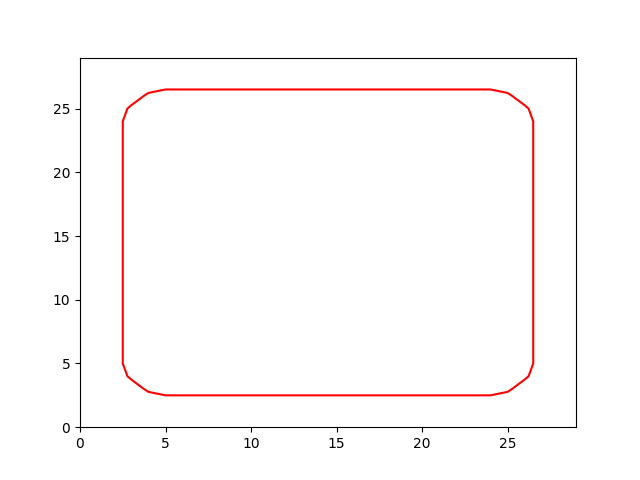
\includegraphics[height=4cm]{img1/level_1_0.png}
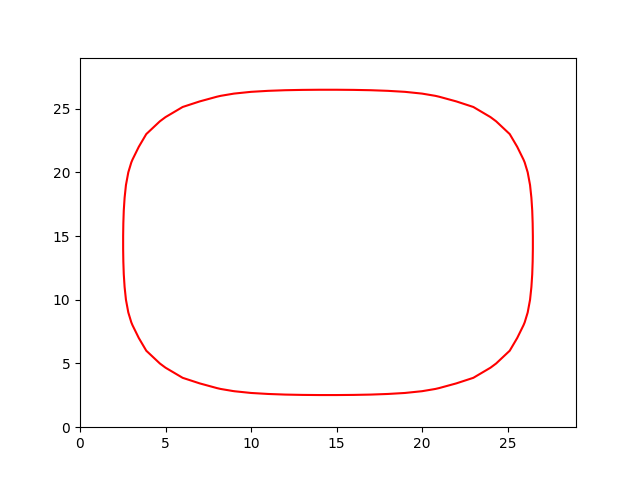
\includegraphics[height=4cm]{img1/level_1_10.png}
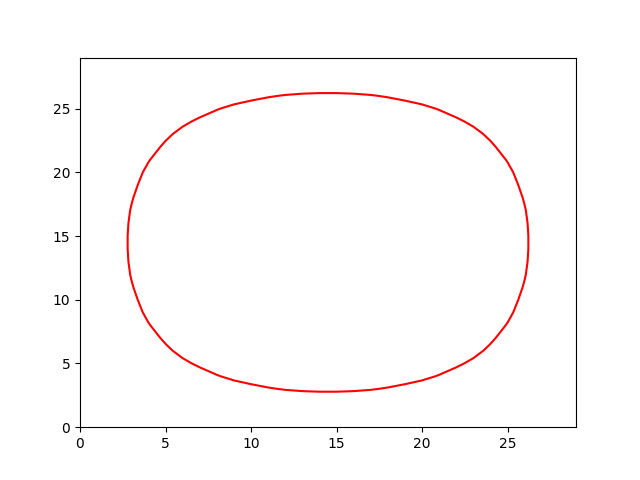
\includegraphics[height=4cm]{img1/level_1_20.png}
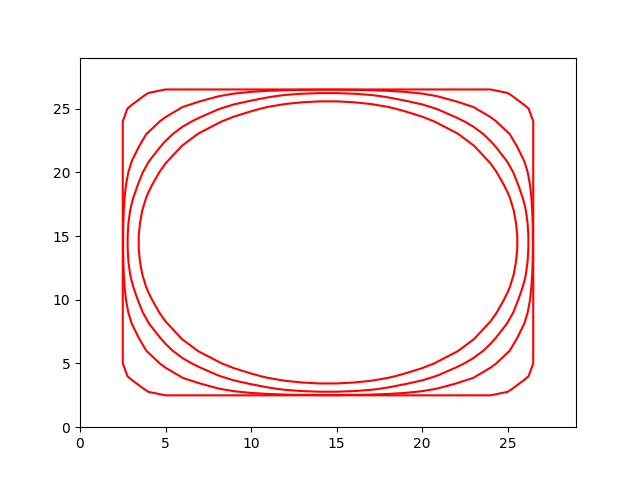
\includegraphics[height=4cm]{img1/level_1_30.png}
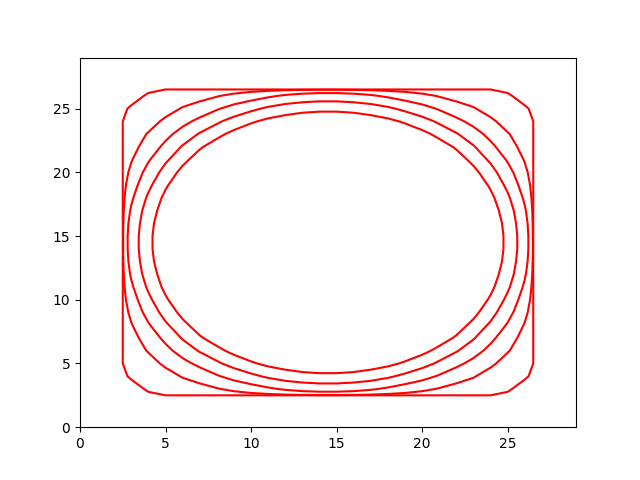
\includegraphics[height=4cm]{img1/level_1_40.png}

İmaj Gruplamak

İmajı bölümlere ayırmak için (segmentation) birkaç faktörün bileşimi
kullanılıyor. Köşeleri kullanan aktif kontur (edge based active contour)
yönteminde ortalama eğim ve imajın piksel değerlerinin farklılıkları (image
gradient) aynı anda kullanılır. Yani kesit seviyesini ilerletirken hızı hem
eğime oranlıyoruz, hem de imaj piksel renk değerleri arasındaki farka ters
oranda hızlandırıyor, ya da yavaşlatıyoruz. Böylece kesit seviyemiz renk
farklılığı çok olmayan yani büyük bir ihtimalle tek bir objeye ait bir
bölgede hızla ilerliyor, büyük renk farkının olduğu büyük bir ihtimalle bir
kenar noktasına gelince ise yavaşlıyor. O sırada kesit seviyesinin geri
kalan tarafları tabii ki başka hızlarda hareket ediyor olabilirler, zaten
işin püf noktası burada, sonunda resim bölgelere ayrılmış oluyor.

Bitirirken önemli gözlemi vurgulayalım. Problemi matematiksel olarak temsil
ederken, hedefe doğru türetirken sürekli (continous) alemde, sürekli,
kesintisiz fonksiyonlarla iş yapıyoruz. Hesaplama anı gelince sürekli
fonksiyonları ayrıksal (discrete) hale çeviriyoruz, işte uygulamalı
matematiğin hesapsal kısmı burada devreye giriyor. Fakat diferansiyel
denklemler, fonksiyonlar, türevler gibi sürekli matematiğin kavramları çok
önemli, bunlar olmasa problemi soyut bir şekilde temsil edemez, ve
basitleştiremezdik. Temel matematiğin kavramlarını kullanırken yüzyılların
matematiksel bilgisi devreye girebiliyor, matematiğin en yoğun şekilde
kullanıldığı fizikten bol bol teknik alınabilir. Yani söylemek istediğimiz
problemi çözmek için hemen kodlamaya başlamıyoruz, düşünsel eylemin önemli
bir kısmı matematiksel formüllerle (belki kalem kağıtla) yapılıyor.

\inputminted[fontsize=\footnotesize]{python}{levelset2o.py}

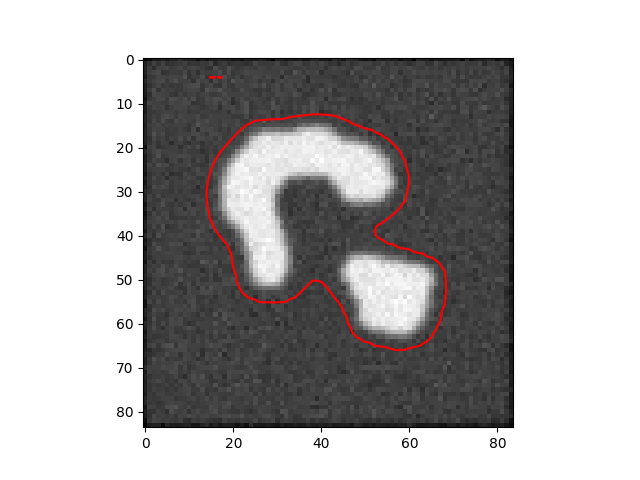
\includegraphics[height=4cm]{img1/level_2_040.png}
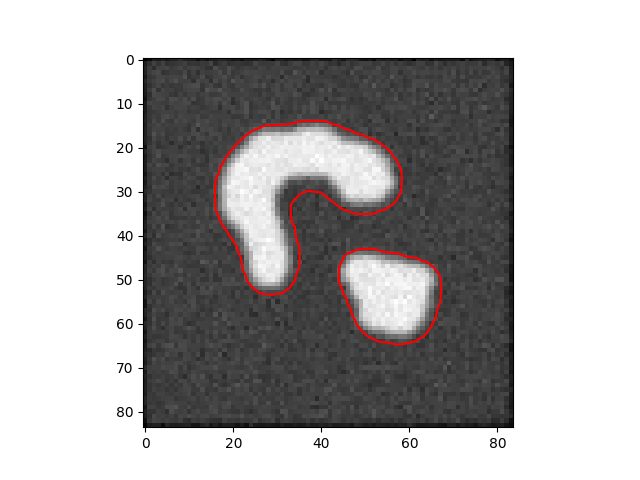
\includegraphics[height=4cm]{img1/level_2_100.png}

Kaynaklar

[1] Courant, {\em Introduction to Calculus and Analysis Volume 2}, sf. 223-232

[2] Wolfram Mathworld, {\em Curvature}, \url{http://mathworld.wolfram.com/Curvature.html}

[3] Strang, {\em Computational Science and Engineering},

[4] Bayramlı, {\em Diferansiyel Denklemler, Türevler}

[5] Kristiadi, {\em Level Set Method Part I: Introduction},
    \url{https://agustinus.kristia.de/techblog/2016/11/05/levelset-method/}

[6] Kristiadi, {\em Level Set Method Part II: Image Segmentation},
    \url{https://agustinus.kristia.de/techblog/2016/11/20/levelset-segmentation/}

[7] Lombaert, {\em Level set method: Explanation},
    \url{https://profs.etsmtl.ca/hlombaert/levelset/}
    
\end{document}




